\documentclass[UTF8,12pt,AutoFakeBold]{ctexbook}

\usepackage{geometry}
\geometry{
	a4paper,
	total={170mm,257mm}, %设置页面尺寸
	left=25mm,
	right=25mm, %奇偶页边距一致
	top=20mm,
	bottom=20mm
}

\usepackage{titlesec}
%改变章节标题样式
\titleformat{\chapter}[block]
{\normalfont\huge\bfseries}{Chapter \thechapter:}{1em}{}

%%%%%%%%%%%%数学%%%%%%%%%%%%%%%%
\usepackage{amsmath, amsfonts, amssymb, amsthm, mathrsfs}
\usepackage{witharrows}
\usepackage{enumitem}
\numberwithin{equation}{section}

%%%%%%%%%%%%表格%%%%%%%%%%%%
\usepackage{multirow, tabularx}

%%%%%%%%%%%%图片%%%%%%%%%%%%	
\usepackage{graphicx, float, subfigure}

%%%%%%%%%%%%算法%%%%%%%%%%%%
\usepackage{algorithm, algpseudocode}

%%%%%%%%%%%%盒子%%%%%%%%%%%%%
\usepackage{tikz, varwidth, mdframed, xcolor}
\usetikzlibrary{calc}
\usepackage[most]{tcolorbox}
\tcbuselibrary{xparse,hooks,skins,breakable,listings}
\input{box.tex}
\def\renewtheorem#1{%
	\expandafter\let\csname#1\endcsname\relax
	\expandafter\let\csname c@#1\endcsname\relax
	\gdef\renewtheorem@envname{#1}
	\renewtheorem@secpar
}
\def\renewtheorem@secpar{\@ifnextchar[{\renewtheorem@numberedlike}{\renewtheorem@nonumberedlike}}
\def\renewtheorem@numberedlike[#1]#2{\newtheorem{\renewtheorem@envname}[#1]{#2}}
\def\renewtheorem@nonumberedlike#1{
	\def\renewtheorem@caption{#1}
	\edef\renewtheorem@nowithin{\noexpand\newtheorem{\renewtheorem@envname}{\renewtheorem@caption}}
	\renewtheorem@thirdpar
}
\def\renewtheorem@thirdpar{\@ifnextchar[{\renewtheorem@within}{\renewtheorem@nowithin}}
\def\renewtheorem@within[#1]{\renewtheorem@nowithin[#1]}

\makeatother

%%%%%%%%%%%%%%%%%%%%
% New environments %
%%%%%%%%%%%%%%%%%%%%

\makeatother
\mdfsetup{skipabove=1em,skipbelow=0em}

\tcbuselibrary{skins}

% Color definitions

\definecolor{proofcolor}{RGB}{0,0,0}

% Dark orange and Dark Red rgb
\definecolor{theorembordercolor}{RGB}{151, 63, 5}
\definecolor{theorembackgroundcolor}{RGB}{248, 241, 234}

\definecolor{examplebordercolor}{RGB}{0, 110, 184}
\definecolor{examplebackgroundcolor}{RGB}{240, 244, 250}

\definecolor{definitionbordercolor}{RGB}{0, 150, 85}
\definecolor{definitionbackgroundcolor}{RGB}{239, 247, 243}

\definecolor{propertybordercolor}{RGB}{128, 0, 128}
\definecolor{propertybackgroundcolor}{RGB}{255, 240, 255}

\definecolor{formulabordercolor}{RGB}{0, 0, 0}
\definecolor{formulabackgroundcolor}{RGB}{230, 229, 245}

\newtheoremstyle{theorem}
{0pt}{0pt}{\normalfont}{0pt}
{}{\;}{0.25em}
{{\sffamily\bfseries\color{theorembordercolor}\thmname{#1}~\thmnumber{\textup{#2}}.}
	\thmnote{\normalfont\color{black}~(#3)}}

\newtheoremstyle{definition}
{0pt}{0pt}{\normalfont}{0pt}
{}{\;}{0.25em}
{{\sffamily\bfseries\color{definitionbordercolor}\thmname{#1}~\thmnumber{\textup{#2}}.}
	\thmnote{\normalfont\color{black}~(#3)}}

\newtheoremstyle{example}
{0pt}{0pt}{\normalfont}{0pt}
{}{\;}{0.25em}
{{\sffamily\bfseries\color{examplebordercolor}\thmname{#1}~\thmnumber{\textup{#2}}.}
	\thmnote{\normalfont\color{black}~(#3)}}

\newtheoremstyle{property}
{0pt}{0pt}{\normalfont}{0pt}
{}{\;}{0.25em}
{{\sffamily\bfseries\color{propertybordercolor}\thmname{#1}~\thmnumber{\textup{#2}}.}
	\thmnote{\normalfont\color{black}~(#3)}}

\newtheoremstyle{formula}
{0pt}{0pt}{\normalfont}{0pt}
{}{\;}{0.25em}
{{\sffamily\bfseries\color{formulabordercolor}\thmname{#1}~\thmnumber{\textup{#2}}.}
	\thmnote{\normalfont\color{black}~(#3)}}

%%%%%%%%%%%%%%%%%%%%%%%%
% Theorem Environments %
%%%%%%%%%%%%%%%%%%%%%%%%

\theoremstyle{theorem}

\newtheorem{theorem}{Theorem}[section]
\newtheorem{postulate}{Postulate}
\newtheorem{conjecture}{Conjecture}
\newtheorem{corollary}{Corollary}
\newtheorem{lemma}{Lemma}
\newtheorem{conclusion}{Conclusion}

\tcolorboxenvironment{theorem}{
	enhanced jigsaw, pad at break*=1mm, breakable,
	left=4mm, right=4mm, top=1mm, bottom=1mm,
	colback=theorembackgroundcolor, boxrule=0pt, frame hidden,
	borderline west={0.5mm}{0mm}{theorembordercolor}, arc=.5mm
}
\tcolorboxenvironment{postulate}{
	enhanced jigsaw, pad at break*=1mm, breakable,
	left=4mm, right=4mm, top=1mm, bottom=1mm,
	colback=theorembackgroundcolor, boxrule=0pt, frame hidden,
	borderline west={0.5mm}{0mm}{theorembordercolor}, arc=.5mm
}
\tcolorboxenvironment{conjecture}{
	enhanced jigsaw, pad at break*=1mm, breakable,
	left=4mm, right=4mm, top=1mm, bottom=1mm,
	colback=theorembackgroundcolor, boxrule=0pt, frame hidden,
	borderline west={0.5mm}{0mm}{theorembordercolor}, arc=.5mm
}
\tcolorboxenvironment{corollary}{
	enhanced jigsaw, pad at break*=1mm, breakable,
	left=4mm, right=4mm, top=1mm, bottom=1mm,
	colback=theorembackgroundcolor, boxrule=0pt, frame hidden,
	borderline west={0.5mm}{0mm}{theorembordercolor}, arc=.5mm
}
\tcolorboxenvironment{lemma}{
	enhanced jigsaw, pad at break*=1mm, breakable,
	left=4mm, right=4mm, top=1mm, bottom=1mm,
	colback=theorembackgroundcolor, boxrule=0pt, frame hidden,
	borderline west={0.5mm}{0mm}{theorembordercolor}, arc=.5mm
}
\tcolorboxenvironment{conclusion}{
	enhanced jigsaw, pad at break*=1mm, breakable,
	left=4mm, right=4mm, top=1mm, bottom=1mm,
	colback=theorembackgroundcolor, boxrule=0pt, frame hidden,
	borderline west={0.5mm}{0mm}{theorembordercolor}, arc=.5mm
}

%%%%%%%%%%%%%%%%%%%%%%%%%%%
% Definition Environments %
%%%%%%%%%%%%%%%%%%%%%%%%%%%

\theoremstyle{definition}
\newtheorem{definition}{Definition}[section]
\newtheorem{review}{Review}

\tcolorboxenvironment{definition}{
	enhanced jigsaw, pad at break*=1mm, breakable,
	left=4mm, right=4mm, top=1mm, bottom=1mm,
	colback=definitionbackgroundcolor, boxrule=0pt, frame hidden,
	borderline west={0.5mm}{0mm}{definitionbordercolor}, arc=.5mm
}
\tcolorboxenvironment{review}{
	enhanced jigsaw, pad at break*=1mm, breakable,
	left=4mm, right=4mm, top=1mm, bottom=1mm,
	colback=definitionbackgroundcolor, boxrule=0pt, frame hidden,
	borderline west={0.5mm}{0mm}{definitionbordercolor}, arc=.5mm
}


%%%%%%%%%%%%%%%%%%%%%%%%
% Example Environments %
%%%%%%%%%%%%%%%%%%%%%%%%

\theoremstyle{example}
\newtheorem{example}{Example}[section]
\newtheorem{remark}{Remark}
\newtheorem{note}{Note}

\tcolorboxenvironment{example}{
	enhanced jigsaw, pad at break*=1mm, breakable,
	left=4mm, right=4mm, top=1mm, bottom=1mm,
	colback=examplebackgroundcolor, boxrule=0pt, frame hidden,
	borderline west={0.5mm}{0mm}{examplebordercolor}, arc=.5mm
}
\tcolorboxenvironment{remark}{
	enhanced jigsaw, pad at break*=1mm, breakable,
	left=4mm, right=4mm, top=1mm, bottom=1mm,
	colback=white, boxrule=0pt, frame hidden,
	borderline west={0.5mm}{0mm}{examplebordercolor}, arc=.5mm
}
\tcolorboxenvironment{note}{
	enhanced jigsaw, pad at break*=1mm, breakable,
	left=4mm, right=4mm, top=1mm, bottom=1mm,
	colback=white, boxrule=0pt, frame hidden,
	borderline west={0.5mm}{0mm}{examplebordercolor}, arc=.5mm
}


%%%%%%%%%%%%%%%%%%%%%%%%%
% Property Environments %
%%%%%%%%%%%%%%%%%%%%%%%%%

\theoremstyle{property}
\newtheorem{property}{Property}[section]
\newtheorem{proposition}{Proposition}[section]

\tcolorboxenvironment{property}{
	enhanced jigsaw, pad at break*=1mm, breakable,
	left=4mm, right=4mm, top=1mm, bottom=1mm,
	colback=propertybackgroundcolor, boxrule=0pt, frame hidden,
	borderline west={0.5mm}{0mm}{propertybordercolor}, arc=.5mm
}
\tcolorboxenvironment{proposition}{
	enhanced jigsaw, pad at break*=1mm, breakable,
	left=4mm, right=4mm, top=1mm, bottom=1mm,
	colback=propertybackgroundcolor, boxrule=0pt, frame hidden,
	borderline west={0.5mm}{0mm}{propertybordercolor}, arc=.5mm
}

%%%%%%%%%%%%
% Formula %
%%%%%%%%%%%%

\theoremstyle{formula}
\newtheorem{formula}{Formula}[section]

\tcolorboxenvironment{formula}{
	enhanced jigsaw, pad at break*=1mm, breakable,
	left=4mm, right=4mm, top=1mm, bottom=1mm,
	colback=formulabackgroundcolor, boxrule=0pt, frame hidden,
	borderline west={0.5mm}{0mm}{formulabordercolor}, arc=.5mm
}

%%%%%%%%%
% Proof %
%%%%%%%%%

% These patches must be placed after \tcolorboxenvironment !
\AddToHook{env/theorem/after}{\colorlet{proofcolor}{theorembordercolor}}
\AddToHook{env/postulate/after}{\colorlet{proofcolor}{theorembordercolor}}
\AddToHook{env/conjecture/after}{\colorlet{proofcolor}{theorembordercolor}}
\AddToHook{env/corollary/after}{\colorlet{proofcolor}{theorembordercolor}}
\AddToHook{env/lemma/after}{\colorlet{proofcolor}{theorembordercolor}}
\AddToHook{env/conclusion/after}{\colorlet{proofcolor}{theorembordercolor}}

\AddToHook{env/definition/after}{\colorlet{proofcolor}{definitionbordercolor}}
\AddToHook{env/review/after}{\colorlet{proofcolor}{definitionbordercolor}}

\AddToHook{env/example/after}{\colorlet{proofcolor}{examplebordercolor}}
\AddToHook{env/remark/after}{\colorlet{proofcolor}{examplebordercolor}}
\AddToHook{env/note/after}{\colorlet{proofcolor}{examplebordercolor}}

\AddToHook{env/property/after}{\colorlet{proofcolor}{propertybordercolor}}
\AddToHook{env/proposition/after}{\colorlet{proofcolor}{propertybordercolor}}

\AddToHook{env/formula/after}{\colorlet{proofcolor}{formulabordercolor}}

\renewcommand{\qedsymbol}{$\square$}
\let\qedsymbolMyOriginal\qedsymbol
\renewcommand{\qedsymbol}{
	\color{proofcolor}\qedsymbolMyOriginal
}

\newtheoremstyle{proof}
{0pt}{0pt}{\normalfont}{0pt}
{}{\;}{0.25em}
{{\sffamily\bfseries\color{proofcolor}\thmname{#1}.}
	\thmnote{\normalfont\color{black}~(\textit{#3})}}

\theoremstyle{proof}
%\renewtheorem{proof}{Proof}

\tcolorboxenvironment{proof}{
	enhanced jigsaw, pad at break*=1mm, breakable,
	left=4mm, right=4mm, top=1mm, bottom=1mm,
	colback=white, boxrule=0pt, frame hidden,
	%borderline west={0.5mm}{0mm}{proofcolor}, arc=.5mm
}

\newenvironment{info}{\begin{tcolorbox}[
		arc=0mm,
		colback=white,
		colframe=gray,
		title=Info,
		fonttitle=\sffamily,
		breakable
		]}{\end{tcolorbox}}
\newenvironment{terminology}{\begin{tcolorbox}[
		arc=0mm,
		colback=white,
		colframe=green!60!black,
		title=Terminology,
		fonttitle=\sffamily,
		breakable
		]}{\end{tcolorbox}}
\newenvironment{warning}{\begin{tcolorbox}[
		arc=0mm,
		colback=white,
		colframe=red,
		title=Warning,
		fonttitle=\sffamily,
		breakable
		]}{\end{tcolorbox}}
\newenvironment{caution}{\begin{tcolorbox}[
		arc=0mm,
		colback=white,
		colframe=yellow,
		title=Caution,
		fonttitle=\sffamily,
		breakable
		]}{\end{tcolorbox}}

\definecolor{citecolor}{RGB}{60,120,216}
\definecolor{urlcolor}{RGB}{60,120,216}
\definecolor{linkcolor}{RGB}{60,120,216}

%%%%%%%%%%%%超链接%%%%%%%%%%%%%
\usepackage{hyperref}
\hypersetup{
	colorlinks=true,
	linkcolor=linkcolor,
	urlcolor=urlcolor,
	%allcolors=blue,
	citecolor=cyan,
	pdftitle={Real Analysis},
	%linkcolor=blue,
	filecolor=magenta,      
	%urlcolor=cyan,
}

%%%%%%%%%%%%参考文献%%%%%%%%%%%%%
\usepackage[round]{natbib}
\bibliographystyle{unsrtnat}

%%%%%%%%%%%%其他%%%%%%%%%%%%%
\usepackage[english]{babel}
\usepackage{caption, marginnote, lipsum, ifthen}

\definecolor{mynotecolor}{rgb}{0.6, 0.4, 0.2}
\newcommand{\mymarginnote}[1]{
	\ifthenelse{\isodd{\value{page}}}
	{\normalmarginpar\marginnote{\textcolor{mynotecolor}{#1}}}
	{\reversemarginpar\marginnote{\textcolor{mynotecolor}{#1}}}
}

\title{Notes of Real Analysis}
\author{Renhe W.}
\date{}

%文章开始部分
\begin{document}
	\maketitle
	\tableofcontents
	
	\newpage
	\kaishu
	%引言
	\section{Introduction}
	This note is to provide an easy understanding of Real Analysis, and to continue to understand and work on more specific areas. And the content are almost come from \href{https://www.bilibili.com/video/BV1FT411C7wM/?spm_id_from=333.337.search-card.all.click&vd_source=ba9c3e9308deddcceb8190c43ed27dfd}{bilibili}
	
	
	\chapter{Abstract Measures}
	\section{Building Block}
	\begin{definition}[closed rectangle]
		A \textbf{closed rectangle} $R$ in $\mathbb{R}^d$ is defined as the Cartesian product of closed intervals. Specifically, $R$ can be written as:
		$$
		R=\left[a_1, b_1\right] \times\left[a_2, b_2\right] \times \cdots \times\left[a_d, b_d\right],
		$$
		where $\left[a_i, b_i\right]$ are closed intervals on the real line, and $a_i \leq b_i$ for all $i$ from 1 to $d$.
		
		In other words,
		$$
		R = \{(X_1,X_2,\dots,X_d)\in\mathbb{R}^d:a_j\leq b_j, j = 1,\dots,d\},
		$$
		The {\color{blue}volume} of $R$ is
		$$
			\left | R \right | = \left(b_1-a_1\right) \times \left(b_2-a_2\right) \times \cdots \times\left(b_d-a_d\right),
		$$
		An \textbf{open rectangle} is the product of open intervals, and the interior of the rectangle $R$ is
		$$
			\left(a_1, b_1\right) \times\left(a_2, b_2\right) \times \cdots \times\left(a_d, b_d\right).
		$$
	\end{definition}
	
	\begin{example}[Closed Rectangles]There are some examples of \textbf{closed rectangle}:
		\begin{enumerate}
			\item  In $\mathbb{R}^2$ (the plane), a building block might be a rectangle defined by $R=[1,3] \times[2,4]$. This rectangle includes all points $(x, y)$ where $1 \leq x \leq 3$ and $2 \leq y \leq 4$.
			\begin{figure}[H] 
				\centering  
			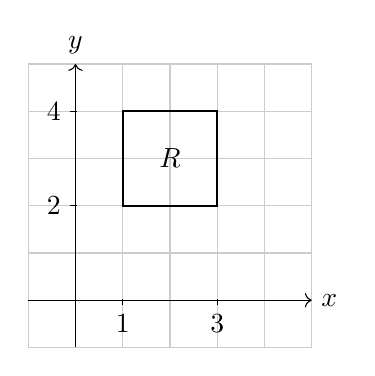
\begin{tikzpicture}[scale=0.6]
				% Draw the axes
				\draw[thin,gray!40] (-1,-1) grid (5,5);
				\draw[->] (-1,0)--(5,0) node[right]{$x$};
				\draw[->] (0,-1)--(0,5) node[above]{$y$};
				
				% Draw the rectangle with points and labels
				\draw[thick] (1,2) rectangle (3,4);
				\foreach \x/\xtext in {1, 3}
				\draw (\x,1pt) -- (\x,-3pt) node[anchor=north] {$\x$};
				\foreach \y/\ytext in {2, 4}
				\draw (1pt,\y) -- (-3pt,\y) node[anchor=east] {$\y$};
				
				% Label the rectangle
				\node at (2,3) {$R$};
			\end{tikzpicture}
			 \caption{The rectangle $R = [1, 3] \times [2, 4]$ in $\mathbb{R}^2$}
			\end{figure}
			\item  In $\mathbb{R}^3$ (three-dimensional space), a typical building block could be a rectangular prism (or box) defined by $R=[0,1] \times[0,1] \times[0,1]$. This includes all points $(x, y, z)$ where $0 \leq x \leq 1,0 \leq y \leq 1$, and $0 \leq z \leq 1$.
		\end{enumerate}
	\end{example}
	
	\begin{definition}[Almost Disjoint]
		A union of rectangles is said to be {\color{blue}almost disjoint} if the interiors of them are disjoint.
	\end{definition}
	
	\begin{figure}[H]
		\centering
		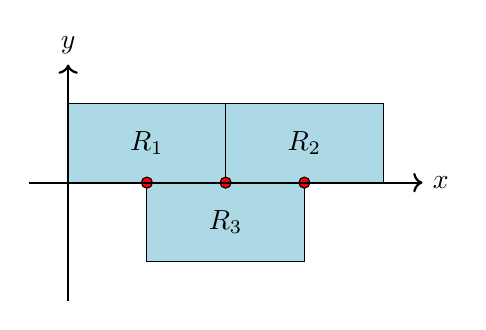
\begin{tikzpicture}
			% Define colors for visibility
			\definecolor{lightblue}{RGB}{173,216,230}
			
			% Draw the first rectangle
			\filldraw[fill=lightblue, draw=black] (0,0) rectangle (2,1);
			\node at (1, 0.5) {$R_1$};
			
			% Draw the second rectangle
			\filldraw[fill=lightblue, draw=black] (2,0) rectangle (4,1);
			\node at (3, 0.5) {$R_2$};
			
			% Draw the third rectangle
			\filldraw[fill=lightblue, draw=black] (1,-1) rectangle (3,0);
			\node at (2, -0.5) {$R_3$};
			
			% Label the touching points
			\draw[fill=red] (2,0) circle (2pt);
			\draw[fill=red] (1,0) circle (2pt);
			\draw[fill=red] (3,0) circle (2pt);
			
			% Draw axes (optional, for reference)
			\draw[thick,->] (-0.5,0) -- (4.5,0) node[right] {$x$};
			\draw[thick,->] (0,-1.5) -- (0,1.5) node[above] {$y$};
		\end{tikzpicture}
	\end{figure}
	The rectangle $R_1$ and $R_2$ share a common boundary along the line $x=2$ but do not overlap. $R_3$ is positioned such that it touches the bottom edges of $R_1$ and $R_2$ at points along the line $y=0$. The points where the rectangles touch are highlighted with red dots to emphasize the boundary interactions but no interior overlap.
	\begin{lemma}
		If a rectangles is the almost disjoint union of finitely many rectangles: $R=\bigcup_{N}^{k=1} R_k $, then $\left | R \right |=\sum_{k=1}^{N}\left | R_k \right |$.
	\end{lemma}
	这个引理描述了一种特殊情况,其中一个矩形 \( R \) 是有限个几乎不相交的矩形的并集,即 \( R=\bigcup_{k=1}^N R_k \),并且这些矩形的内部不相交. 在这种情况下,\( R \) 的体积等于所有这些子矩形体积的总和.
	\begin{proof}
		定义每个 \( R_k \) 为闭矩形 \([a_{k1}, b_{k1}] \times [a_{k2}, b_{k2}] \times \cdots \times [a_{kd}, b_{kd}]\), 对于任何 \( i \neq j \),\( \text{int}(R_i) \cap \text{int}(R_j) = \emptyset \). \marginnote{\tiny Almost Disjoint}其中每个 \( R_k \) 的体积计算为 \( |R_k| = \prod_{j=1}^d (b_{kj} - a_{kj}) \).
		
		设 \( R = [a_1, b_1] \times [a_2, b_2] \times \cdots \times [a_d, b_d] \),其中 \( a_j = \min_k a_{kj} \),\( b_j = \max_k b_{kj} \)\marginnote{\tiny 最小包含矩形 \( R \)}.
		
		由于 \( \text{int}(R_i) \cap \text{int}(R_j) = \emptyset \),可以断定每个 \( R_k \) 的体积贡献是独立的,即它们的体积之和给出了 \( R \) 中被覆盖的全部体积.
		
		\( R_k \) 的边界可能与其他 \( R_k \) 的边界重合,但由于边界的测度在整体测度中不起主导作用(在高维中测度为零),因此不影响总体积计算.
		
		因此,可以通过各 \( R_k \) 的体积独立累加,无需减去重叠部分,从而得到 \( R \) 的总体积,即 \( |R| = \sum_{k=1}^N |R_k| \).
	\end{proof}
	
	\begin{lemma}
		If $R, R_1,\dots, R_N$ are rectangles, and $R \subset \bigcup_{}^{}$
		
	\end{lemma}
	
	
\end{document}